\chapter{Opis projektnog zadatka}
		
		\large Cilj ovog projekta je razviti programsku podršku za izradu web
aplikacije koja će korisnicima omogućiti objaviti ili pronaći događaj
u svojoj zajednici. U aplikaciji će organizatori događanja postavljati
najave za događanja koja organiziraju, a zainteresirani posjetitelji će
moći najaviti svoj dolazak te pisati recenzije. 

Kako bi korisnik pristupio funkcionalnostima aplikacije, prvo će se trebati registrirati kao posjetitelj ili kao organizator. Organizatori će svoja događanja koja promoviraju putem aplikacije moći naplaćivati ili ne naplaćivati. Ako organizatori naplaćuju svoja događanja, plaćat će korištenje aplikacije na mjesečnoj bazi. To će raditi putem PayPala ili pomoću kreditnih kartica. Za razliku od njih, posjetitelji i organizatori beplastnih događanja koristit će aplikaciju besplatno.

Posjetitelji će nakon pokretanja aplikacije moći vidjeti popis događanja u odredenom vremenskom razdoblju koje sami odaberu (24h, 7 dana ili 30 dana). Svako događanje imat će definirano mjesto, vrijeme, trajanje i cijenu ulaznice (ukoliko se radi o događanju koje se plaća). Za svako prikazano događanje, korisnik će moći izjasniti svoj interes: “dolazim”, “ne dolazim” ili “možda dolazim”. Bit će ostvarena i funkcionalnost koja posjetiteljima omogućuje da se predomisle i promijene status svog interesa. Korisnik će također moći napisati recenziju za svako prikazano događanje koje se održalo u posljednjih 48 sati. Također, posjetitelji će moći postaviti kriterije po vrsti događanja i lokaciji te primati notifikacije kad bude objavljen događaj koji ih zadovoljava.

	Na javnim profilima organizatora nalazit će se osnovne informacije o njima, poput naziva, adrese i dodatnih linkova. Na njihovim će profilima biti prikazana i sva događanja koja su organizirali u zadnje dvije godine. Za svako događanje dostupne su dodatne informacije poput naziva, vrste, lokacije, vremena početka, trajanja i galerija fotografija i videa. Takve informacije organizator postavlja sam. Za svaki protekli događaj bit će dostupne i korisničke recenzije, a za svaki tek najavljeni bit će moguće vidjeti koliko ljudi planira doći.
 
	U sustavu će postojati i administratori čija je funkcija postavljanje cijene članstva.

Ovakva aplikacija bila bi korisna za oglašavanje događaja koji su ograničeni svojom temom, grupom uzvanika ili lokacijom. Za događaje širih parametara, platforma poput Facebooka ili Instagrama je idealna, ali bi ovakva aplikacija odarbirom teme na koju želi suziti svoje događaje mogla postati korisnija korisnicima zainteresiranim za tu temu. Primijenjena na FER-ovce mogla bi služiti oglašavanju natjecanja iz programiranja u Hrvatskoj, a primijenjena na likovne umjetnike mogla bi služiti oglašavanju izložbi. S druge strane, mogla bi biti korisna i odabirom grupe uzvanika umjesto odabirom teme događaja. Npr., mogla bi služiti tome da zaposlenici neke veće firme lakše saznaju za aktivnosti koje su im dostupne kao zaposlenicima te firme. Također bi bila korisna i sužavanjem lokacije samih evenata. Npr., kompleks poput velesajma mogao bi dopuštati organizatorima da oglašavaju svoje događaje koji će se tamo odvijati.

Za slične se svrhe dosad koristio Facebook, ali zbog zakrčenosti platforme i zbog tog a što joj organizacija i oglašavanje događanja nije primarna svrha, potrebne su aplikacije koje se bave baš isključivo time. Nekoliko popularnih aplikacija takve vrste su Eventbrite i Bizzabo. Osim samog oglašavanja, obje aplikacije nude i mogućnost prodaje karata online, a organizator prijavljen u aplikaciju ima i mogućnost skeniranja karata i vođenja evidencije gostiju. Ovakve aplikacije imaju neke dodatne mogućnosti u odnosu na cilj ovog projekta jer se fokusiraju na pružanje usluge Samim organizatorima, dok se u ovom projektu stavlja naglasak na samo oglašavanje i promociju događanja.
			
		
		\textbf{\textit{dio 1. revizije}}\\
		
		\textit{Na osnovi projektnog zadatka detaljno opisati korisničke zahtjeve. Što jasnije opisati cilj projektnog zadatka, razraditi problematiku zadatka, dodati nove aspekte problema i potencijalnih rješenja. Očekuje se minimalno 3, a poželjno 4-5 stranica opisa.	Teme koje treba dodatno razraditi u ovom poglavlju su:}
		\begin{packed_item}
			\item \textit{potencijalna korist ovog projekta}
			\item \textit{postojeća slična rješenja (istražiti i ukratko opisati razlike u odnosu na zadani zadatak). Dodajte slike koja predočavaju slična rješenja.}
			\item \textit{skup korisnika koji bi mogao biti zainteresiran za ostvareno rješenje.}
			\item \textit{mogućnost prilagodbe rješenja }
			\item \textit{opseg projektnog zadatka}
			\item \textit{moguće nadogradnje projektnog zadatka}
		\end{packed_item}
		
		\textit{Za pomoć pogledati reference navedene u poglavlju „Popis literature“, a po potrebi konzultirati sadržaj na internetu koji nudi dobre smjernice u tom pogledu.}
		\eject
		
		\section{Primjeri u \LaTeX u}
		
		\textit{Ovo potpoglavlje izbrisati.}\\

		U nastavku se nalaze različiti primjeri kako koristiti osnovne funkcionalnosti \LaTeX a koje su potrebne za izradu dokumentacije. Za dodatnu pomoć obratiti se asistentu na projektu ili potražiti upute na sljedećim web sjedištima:
		\begin{itemize}
			\item Upute za izradu diplomskog rada u \LaTeX u - \url{https://www.fer.unizg.hr/_download/repository/LaTeX-upute.pdf}
			\item \LaTeX\ projekt - \url{https://www.latex-project.org/help/}
			\item StackExchange za Tex - \url{https://tex.stackexchange.com/}\\
		
		\end{itemize} 	


		
		\noindent \underbar{podcrtani tekst}, \textbf{podebljani tekst}, 	\textit{nagnuti tekst}\\
		\noindent \normalsize primjer \large primjer \Large primjer \LARGE {primjer} \huge {primjer} \Huge primjer \normalsize
				
		\begin{packed_item}
			
			\item  primjer
			\item  primjer
			\item  primjer
			\item[] \begin{packed_enum}
				\item primjer
				\item[] \begin{packed_enum}
					\item[1.a] primjer
					\item[b] primjer
				\end{packed_enum}
				\item primjer
			\end{packed_enum}
			
		\end{packed_item}
		
		\noindent primjer url-a: \url{https://www.fer.unizg.hr/predmet/proinz/projekt}
		
		\noindent posebni znakovi: \# \$ \% \& \{ \} \_ 
		$|$ $<$ $>$ 
		\^{} 
		\~{} 
		$\backslash$ 
		
		
		\begin{longtblr}[
			label=none,
			entry=none
			]{
				width = \textwidth,
				colspec={|X[8,l]|X[8, l]|X[16, l]|}, 
				rowhead = 1,
			} %definicija širine tablice, širine stupaca, poravnanje i broja redaka naslova tablice
			\hline \SetCell[c=3]{c}{\textbf{naslov unutar tablice}}	 \\ \hline[3pt]
			\SetCell{LightGreen}IDKorisnik & INT	&  	Lorem ipsum dolor sit amet, consectetur adipiscing elit, sed do eiusmod  	\\ \hline
			korisnickoIme	& VARCHAR &   	\\ \hline 
			email & VARCHAR &   \\ \hline 
			ime & VARCHAR	&  		\\ \hline 
			\SetCell{LightBlue} primjer	& VARCHAR &   	\\ \hline 
		\end{longtblr}
		

		\begin{longtblr}[
				caption = {Naslov s referencom izvan tablice},
				entry = {Short Caption},
			]{
				width = \textwidth, 
				colspec = {|X[8,l]|X[8,l]|X[16,l]|}, 
				rowhead = 1,
			}
			\hline
			\SetCell{LightGreen}IDKorisnik & INT	&  	Lorem ipsum dolor sit amet, consectetur adipiscing elit, sed do eiusmod  	\\ \hline
			korisnickoIme	& VARCHAR &   	\\ \hline 
			email & VARCHAR &   \\ \hline 
			ime & VARCHAR	&  		\\ \hline 
			\SetCell{LightBlue} primjer	& VARCHAR &   	\\ \hline 
		\end{longtblr}
	


		
		
		%unos slike
		\begin{figure}[H]
			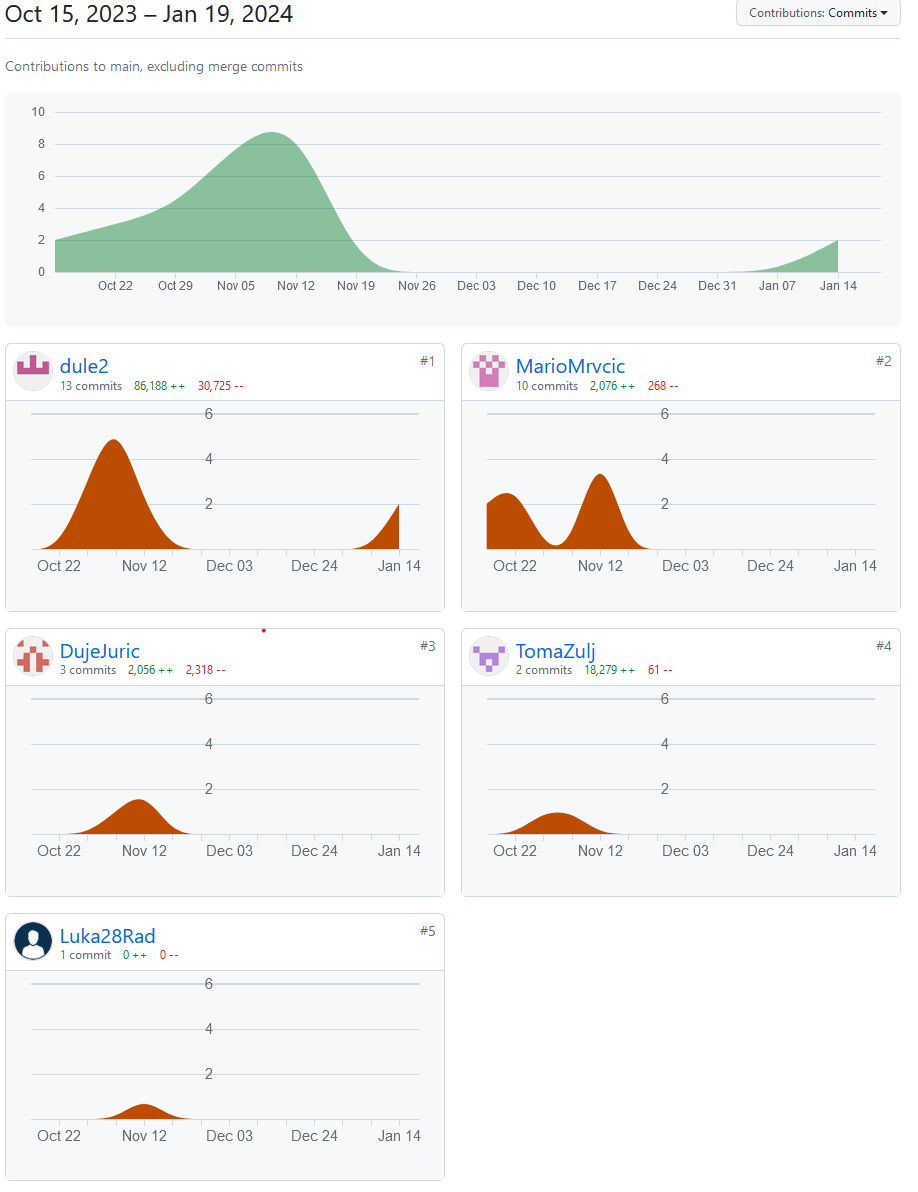
\includegraphics[scale=0.4]{slike/aktivnost.PNG} %veličina slike u odnosu na originalnu datoteku i pozicija slike
			\centering
			\caption{Primjer slike s potpisom}
			\label{fig:promjene}
		\end{figure}
		
		\begin{figure}[H]
			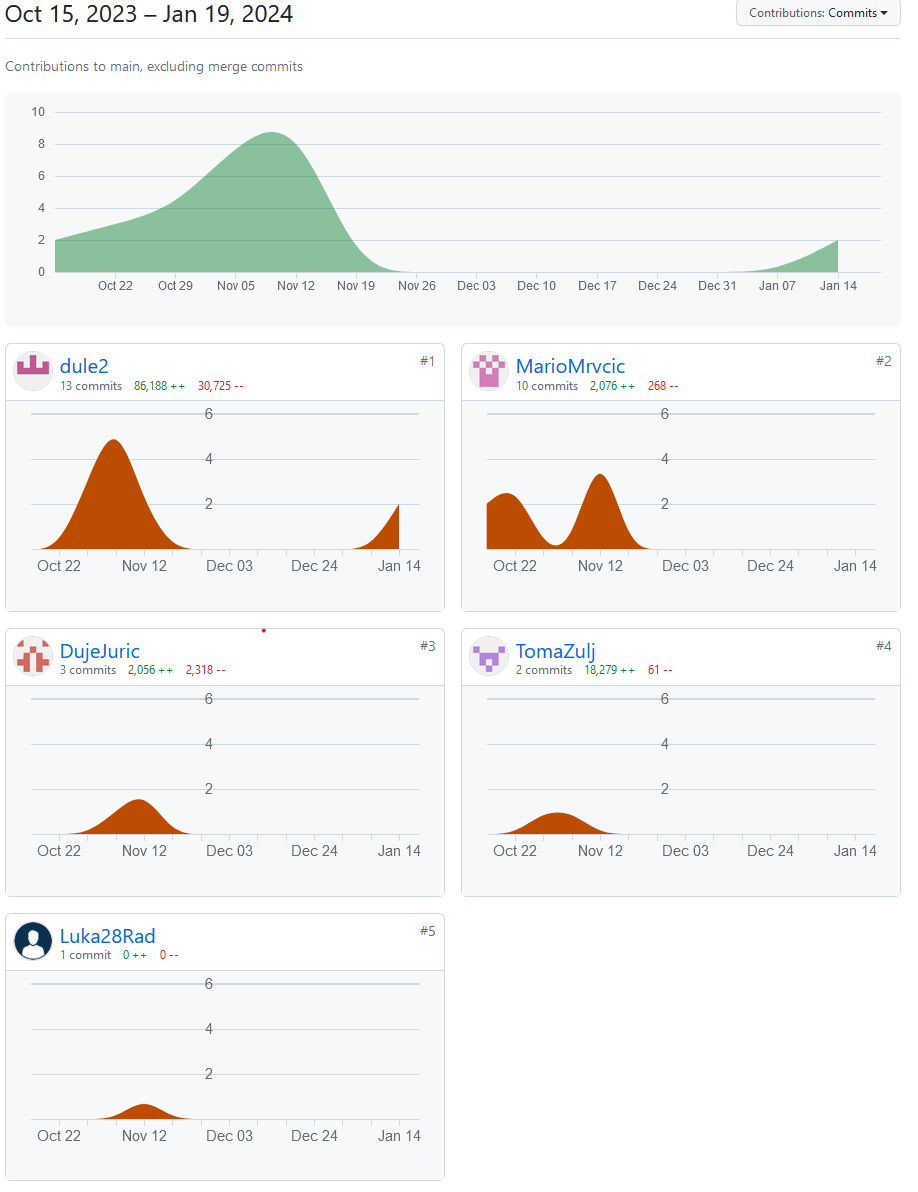
\includegraphics[width=\textwidth]{slike/aktivnost.PNG} %veličina u odnosu na širinu linije
			\caption{Primjer slike s potpisom 2}
			\label{fig:promjene2} %label mora biti drugaciji za svaku sliku
		\end{figure}
		
		Referenciranje slike \ref{fig:promjene2} u tekstu.
		
		\eject
		
	